%*******************************************************
% Appendix - CBF algorithm
%*******************************************************


\chapter{Appendix}\label{ch:appendix} 

\section{Questionnaire}
\begin{figure}[H]
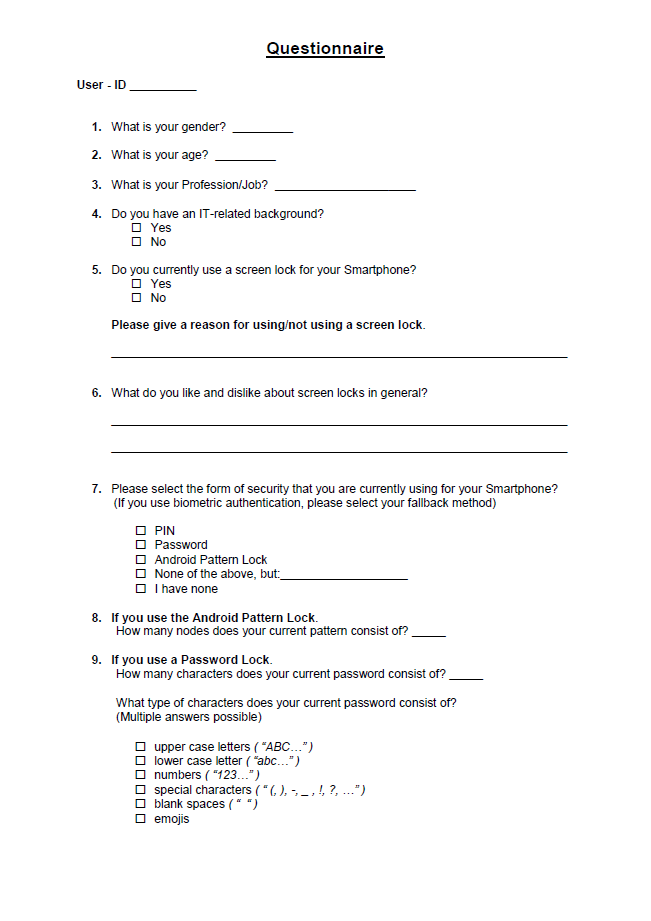
\includegraphics[width=13cm, height=17cm]{Chapters/graphics/survey1.PNG}
\caption{Questionnaire to our study, page 1.}
\label{fig:survey1}
\end{figure}

\begin{figure}[H]
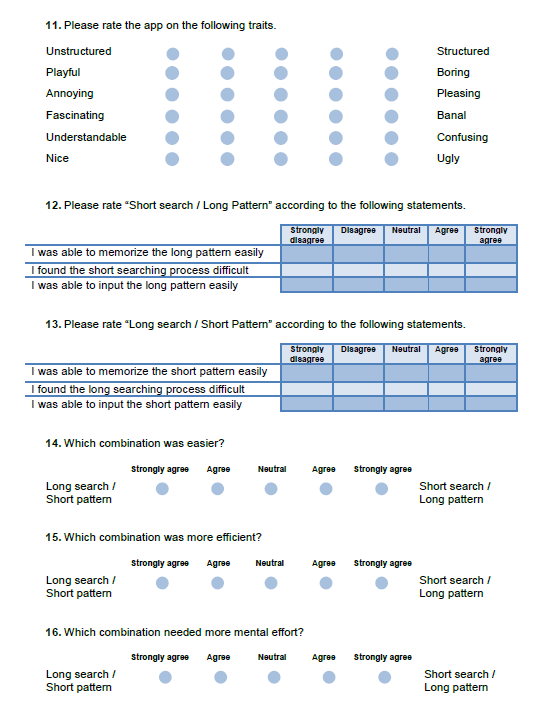
\includegraphics[width=13cm, height=17cm]{Chapters/graphics/survey2.PNG}
\caption{Questionnaire to our study, page 2. In the survey ratios were referred to as "combinations" for easier understanding. Refer to figure \ref{fig:illustration} to understand the used descriptions of for each ratio.}
\label{fig:survey2}
\end{figure}

\begin{figure}[H]
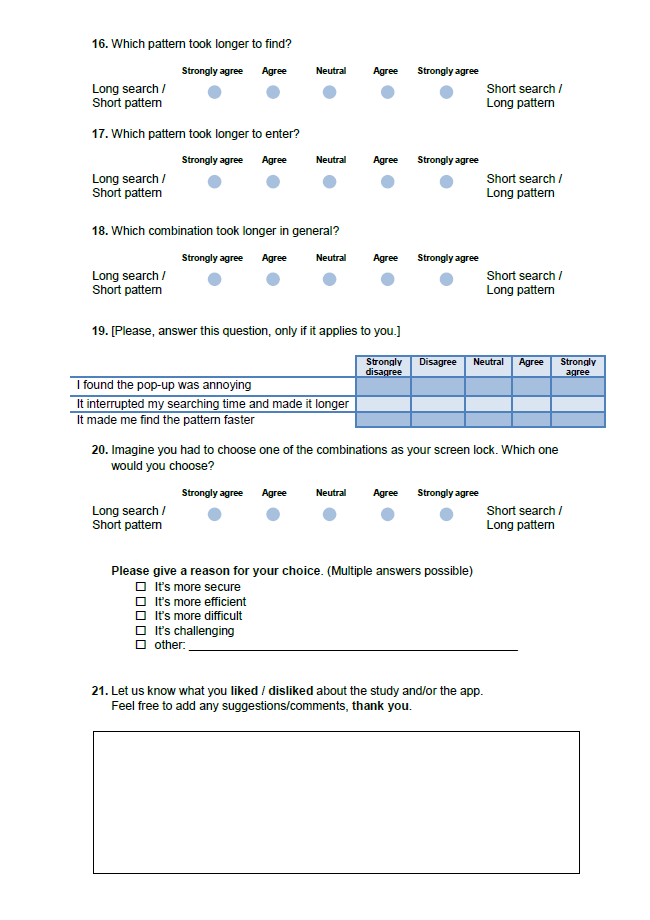
\includegraphics[width=13cm, height=17cm]{Chapters/graphics/survey3.PNG}
\caption{Questionnaire to our study, page 3. In the survey ratios were referred to as "combinations" for easier understanding. Refer to figure \ref{fig:illustration} to understand the used descriptions of for each ratio.}
\label{fig:survey3}
\end{figure}

\section{Illustration}

\begin{figure}[H]
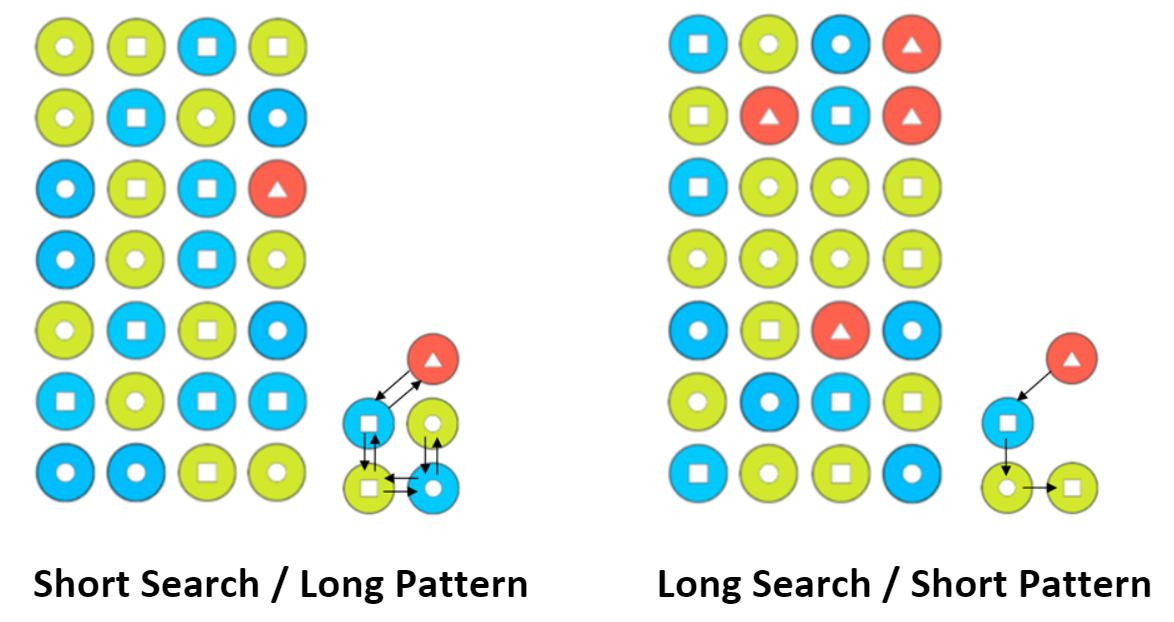
\includegraphics[width=15cm, height=10cm]{Chapters/graphics/illustration.PNG}
\caption{This is an illustration which was given to the participants as an aid to help them remember the contrasting ratios, as they filled out the questionnaires. The description of the ratios was simplified for easier understanding: \textit{short orientation/long input} (Left), \textit{long orientation/short input} (Right).}
\label{fig:illustration}
\end{figure}




